\documentclass{article}
\usepackage{pgfplots}
\pgfplotsset{compat=1.16}

\begin{document}

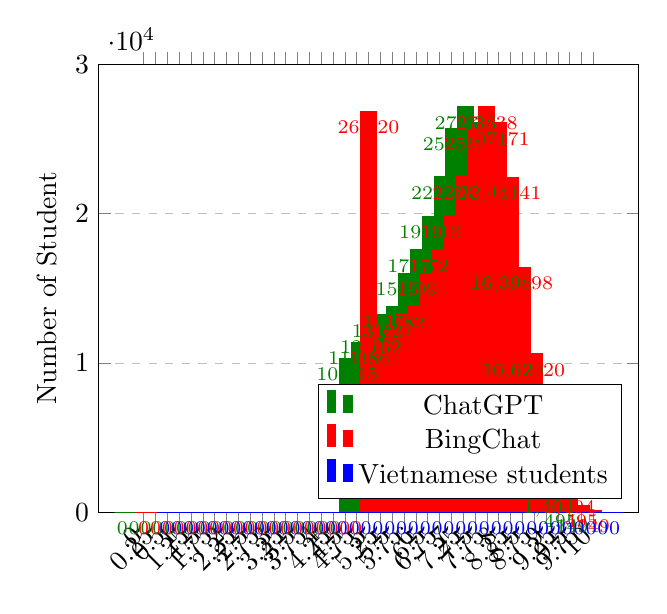
\begin{tikzpicture}
    \begin{axis}[
        ybar,
        bar width=0.2cm,
        ymin=0,
        ymax=30000,
        ylabel={Number of Student},
        xlabel={},
        symbolic x coords={0, 0.25, 0.5, 1, 1.25, 1.5, 1.75, 2, 2.25, 2.5, 2.75, 3, 3.25, 3.5, 3.75, 4, 4.25, 4.5, 4.75, 5, 5.25, 5.5, 5.75, 6, 6.5, 6.75, 7, 7.25, 7.5, 7.75, 8, 8.25, 8.5, 8.75, 9, 9.25, 9.5, 9.75, 10},
        xtick=data,
        nodes near coords,
        every node near coord/.append style={anchor=north, font=\scriptsize},
        x tick label style={rotate=45, anchor=east},
        legend pos=south east,
        ymajorgrids=true,
        grid style=dashed,
    ]
    
    \addplot[green!50!black, fill=green!50!black] coordinates {(0, 0) (0.25, 0) (0.5, 0) (1, 0) (1.25, 0) (1.5, 0) (1.75, 0) (2, 0) (2.25, 0) (2.5, 0) (2.75, 0) (3, 0) (3.25, 0) (3.5, 0) (3.75, 0) (4, 0) (4.25, 0) (4.5, 0) (4.75, 0) (5, 10315) (5.25, 11386) (5.5, 12162) (5.75, 13227) (6, 13782) (6.5, 15999) (6.75, 17572) (7, 19818) (7.25, 22463) (7.5, 25721) (7.75, 27138) (8, 26071) (8.25, 22441) (8.5, 16398) (8.75, 10620) (9, 5998) (9.25, 3051) (9.5, 1404) (9.75, 495) (10, 149)};
    \addplot[red, fill=red] coordinates {(0, 0) (0.25, 0) (0.5, 0) (1, 0) (1.25, 0) (1.5, 0) (1.75, 0) (2, 0) (2.25, 0) (2.5, 0) (2.75, 0) (3, 0) (3.25, 0) (3.5, 0) (3.75, 0) (4, 0) (4.25, 0) (4.5, 0) (4.75, 0) (5, 26820) (5.25, 11386) (5.5, 12162) (5.75, 13227) (6, 13782) (6.5, 15999) (6.75, 17572) (7, 19818) (7.25, 22463) (7.5, 25721) (7.75, 27138) (8, 26071) (8.25, 22441) (8.5, 16398) (8.75, 10620) (9, 5998) (9.25, 3051) (9.5, 1404) (9.75, 495) (10, 149)};
    \addplot[blue, fill=blue] coordinates {(0, 0) (0.25, 0) (0.5, 0) (1, 0) (1.25, 0) (1.5, 0) (1.75, 0) (2, 0) (2.25, 0) (2.5, 0) (2.75, 0) (3, 0) (3.25, 0) (3.5, 0) (3.75, 0) (4, 0) (4.25, 0) (4.5, 0) (4.75, 0) (5, 0) (5.25, 0) (5.5, 0) (5.75, 0) (6, 0) (6.5, 0) (6.75, 0) (7, 0) (7.25, 0) (7.5, 0) (7.75, 0) (8, 0) (8.25, 0) (8.5, 0) (8.75, 0) (9, 0) (9.25, 0) (9.5, 0) (9.75, 0) (10, 0)};
    
    \legend{ChatGPT, BingChat, Vietnamese students}
    
    \end{axis}
\end{tikzpicture}

\end{document}